\documentclass{article}
\usepackage[usenames,dvipsnames]{color}
\usepackage{hw}
\usepackage{bm}
\usepackage{amsmath}
\usepackage{graphicx}
\usepackage[colorlinks=true,urlcolor=blue]{hyperref}
\usepackage{geometry}
\geometry{margin=1in}
\usepackage{float}
\setlength{\marginparwidth}{2.15cm}
\usepackage{booktabs}
%\usepackage{enumitem}
\usepackage{epsfig}
\usepackage{setspace}
\usepackage{parskip}
\usepackage{bbm}
\usepackage[]{algorithm2e}
\usepackage{comment}
\usepackage{pdfpages}
\usepackage{physics}
\usepackage{ulem}
\usepackage{hyperref}
\usepackage{macro}
\usepackage{enumerate}
\usepackage{mcode}
\usepackage{soul}

\title{mlsp - hw1 - 2018}
\author{abelinoj }
\date{September 2018}

\begin{document}

\begin{center}
  \centerline{\textsc{\LARGE Homework 1}}
  \vspace{0.5em}
  \centerline{\textsc{\Large Linear Algebra}}
  \vspace{1em}
  \textsc{\large CMU 11-755/18-797: Machine Learning for Signal Processing (Fall 2020)} \\
  \vspace{1em}
  \centerline{OUT: September 10th, 2020}
  \centerline{DUE: {\bf September 21st, 11:59 PM}}
\end{center}
\graphicspath{images}


\section*{START HERE: Instructions}


\begin{itemize*}

\item \textbf{Collaboration policy:} Collaboration on solving the homework is allowed, after you have thought about the problems on your own.  It is also OK to get clarification (but not solutions) from books or online resources, again after you have thought about the problems on your own.  There are two requirements: first, cite your collaborators fully and completely (e.g., ``Jane explained to me what is asked in Question 3.4'').  Second, write your solution {\em independently}: close the book and all of your notes, and send collaborators out of the room, so that the solution comes from you only.


\vspace{0.1in}
\item\textbf{Submitting your work:} Assignments should be submitted as PDFs using Canvas unless explicitly stated otherwise.  Please submit all results as \texttt{report\underline{ }\{YourAndrewID\}.pdf} in you submission.
\textbf{Each derivation/proof should be completed on a separate page}. Submissions can be handwritten, but should be labeled and clearly legible.  Else, submissions can be written in LaTeX.  Upon submission, label each question using the template provided by Canvas. Please refer to Piazza for detailed instruction for joining Canvas and submitting your homework.

\vspace{0.1in}
\item \textbf{Programming}: All programming portions of the assignments should be submitted to Canvas as well.  Please \texttt{zip} all the code and output files together, and submit the compressed file together with the pdf report. We will not be using this for autograding, %but rather for plagiarism detection, 
meaning you may use any programming language you desire.
\end{itemize*}

\newpage
\section{Linear Algebra}
\subsection{Rotational Matrices}
\begin{enumerate}
\item  A rotation in 3-D space (whose coordinates we will call X, Y, Z) is characterized by three angles. We will characterize them as a rotation around the x-axis, a rotation around the y-axis, and a rotation around the z-axis. \\
Derive the rotation matrix $R_1$ that transforms a vector $[x,y,z]^{T}$  to a new vector $[\hat{x},\hat{y},\hat{z}]^{T}$ by rotating it counterclockwise by angle $\theta$ around the x-axis, then an angle $\delta$ around the y-axis, and finally an angle $\phi$ around the z-axis.\\
Derive the rotation matrix $R_2$ that transforms a vector $[x,y,z]^{T}$  to a new vector $[\hat{x},\hat{y},\hat{z}]^{T}$ by rotating it counterclockwise by an angle $\delta$ around the y-axis, then an angle $\theta$ around the x-axis, and finally an angle $\phi$ around the z-axis.

\item Confirm that $R_1R_1^{T} = R_2R_2^{T} = I$
\end{enumerate}






\section{Moore-Penrose Inverse}
The pseudoinverse we covered in lecture is more formally known as the Moore-Penrose inverse. The Moore-Penrose inverse was independently discovered throughout the 20th century. Its name is due to E.H. Moore, an influential mathematician and first head of the mathematics department at the University of Chicago, and Roger Penrose, a mathematician and physicist with too many awards to count.

In lecture, we covered two pseudoinverses for two different cases. The one which we will explore here is the pseudoinverse for the under-determined case:
\[\textrm{Pinv}(T) = T^T(TT^T)^{-1}.\]

\subsection{Moore-Penrose Conditions}

Wikipedia defines the pseudoinverse of $A\in\mathbb{K}^{m\times n}$ as $A^+ \in \mathbb{K}^{n \times m}$ which satisfies:
\begin{enumerate}
    \item $A A^+ A = A$
    \item $A^+ A A^+ = A^+$
    \item $(A A^+)^* = A A^+$
    \item $(A^+ A)^* = A^+ A$
\end{enumerate}
Here, $A^*$ refers to the conjugate transpose of $A$. Wikipedia assumes that $A$ is defined over a given field $\mathbb{K}$; however, we will restrict our discussion and this problem to $\mathbb{R}$, the field of real numbers. In this case, the conjugate transpose becomes regular matrix transposition. The four conditions above are referred to as the Moore-Penrose conditions.

\bigskip

\noindent Using our definition of the pseudoinverse for the under-determined case, verify that each of the Moore-Penrose conditions holds.

\subsection{Pinv and SVD}
The pseudo-inverse of a matrix can be calculated via singular value decomposition. If we represent a matrix $A$ as $A = U \Sigma V^{*}$, then you can show that $A^{+} = V\Sigma^{+}U^*.$ The popular Python package Numpy uses this fact to calculate the pseudoinverse.

\bigskip
\noindent Show that the pseudoinverse of $A$ can be computed by $A^{+} = V\Sigma^{+}U^*.$ That is, show that each of the Moore-Penrose conditions hold when we define the pseudoinverse of $A$ as above. Here, $U, \Sigma,$ and $V$ are all the usual components from singular value decomposition. Please provide at least one reason why this may be a good implementation.

\textbf{N.B.:} In this problem, you will see that a lot of quantities either cancel out or become the identity matrix. In your homework submission, you need to clearly explain why a given quantity would reduce to the identity matrix or cancel out. For example, saying ``$BB^T = I$" will not get you any points. Instead, saying ``$BB^T = I$ since $B$ is an orthogonal matrix, and the inverse of an orthogonal matrix is its transpose" will not only get you points but it will also make the course staff smile.

\subsection{Bonus problem: SVD}

Singular Value Decomposition decomposes any matrix $X$ as 
\[
X = U S V^\top,
\]
where $V$ is the matrix of right singular vectors, $U$ is the matrix of left singular vectors, and $S$ is a diagonal matrix of singular values.  We learned how to interpret these in class.

Let $V_i$ represent the columns of $V$, $U_i$ be the columns of $U$, and $S_i$ be the $i^{\rm th}$ diagonal entry of $S$. By the definition of SVD, $\|V_i\|^2 = 1$, and $V_i^\top V_j = 0\,\forall \,i\neq j$, i.e. the right singular vectors are orthonormal.  Similarly the left singular vectors too are orthonormal, i.e.  $\|U_i\|^2 = 1$, and $U_i^\top U_j = 0\,\forall \,i\neq j$. 

When $X$ is viewed as a data-container matrix the ``energy'' in the data is given by $Egy(X) = \sum_{i,j}X_{ij}^2$, where $X_{ij}$ is the $(i,j)^{\rm th}$ entry of $X$.

Show that 
\[
Egy(X) = \sum_{i} S_i^2.
\]

Hint: $Egy(X) = trace(X^\top X).$

\newpage
\section{Music Transcription}

\subsection{Projection}
 The song ``Polyushka Poly'' is played on the harmonica, the file name of the audio recording is  \texttt{\textbf{polyushka.wav}}, which can be found in the folder \texttt{\textbf{hw1materials}}. It has been downloaded from YouTube with permission from the artist.
\\
\\
A set of notes from a harmonica can be found in folder \texttt{\textbf{hw1materials/note15}}. You are required to transcribe the music. For transcription you must determine how each of the notes is played to compose the music.
\\
\\
You need to compute the spectrogram of the music file using your language/toolbox of choice, such as python (Librosa) or Matlab. First, read and load the audio file at 16000 Hz sample rate. 

% If you are using Matlab, you can use the following command:
% \begin{lstlisting}
% [s,fs] = audioread('filename');
% s = resample(s, 16000,fs);
% \end{lstlisting}

If you are using Python, you can use Librosa to load the wav file as follows (we also recommend using the \texttt{numpy} package for matrix operations below if you use python):

\begin{lstlisting}
import librosa
audio, sr = librosa.load(filename, sr = 16000)
\end{lstlisting}

Next, we can compute the complex Short-Time Fourier Transform (STFT) of the signal \textit{s} and its magnitude spectrogram. Use 2048 sample windows, which correspond to 64 ms analysis windows; overlap/hop length of 256 samples to 64 frames by second of signal. Different toolboxes should provide similar spectrograms. If you are using the Python Librosa library, you can use the following command:


% \begin{lstlisting}
% spectrogram = stft(s',2048,256,0,hann(2048));
% M = abs(spectrogram);
% phase = spectrogram./(M + eps);
% \end{lstlisting}

\begin{lstlisting}
spectrogram = librosa.stft(audio, n_fft=2048, hop_length=256, center=False, win_length=2048)
M = abs(spectrogram)
phase = spectrogram/(M + 2.2204e-16)
\end{lstlisting}

In this case, ${\bf M}$ represents the music file and should be a matrix of $1025 \times 8869$, where the rows correspond to the frequencies and the columns to time. A visualization (Librosa - specshow) of this matrix (spectrogram) should look like the following figure.
\begin{center}
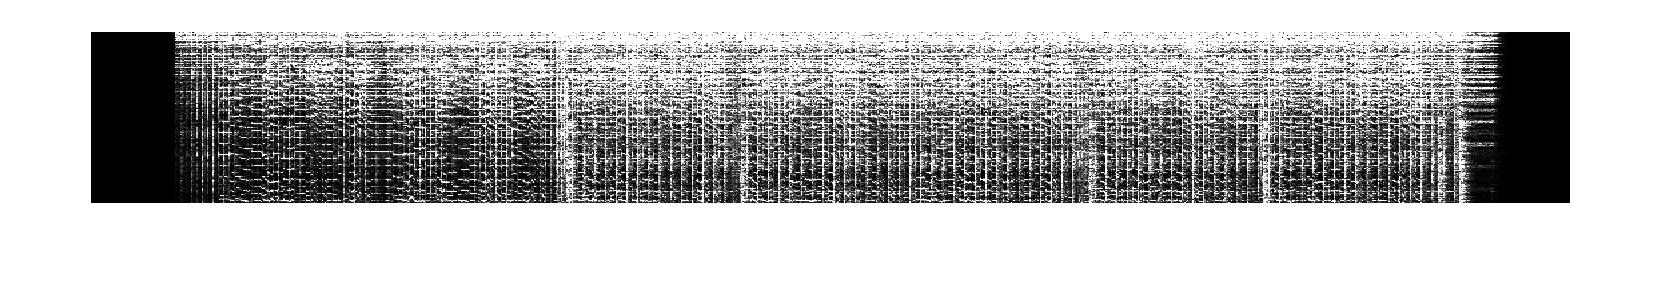
\includegraphics[trim={3cm 0 0 0},clip,scale=0.32]{figs/spectrogram.jpg}
\end{center}
To represent notes, you also need to compute the spectrogram of each note file. However, unlike the music file, we need to represent the matrix just as a one column vector. Hence, we can choose only one vector, or compute the mean of the matrix across time, etc. In this example, we select the middle column:
%[s, fs] = audioread('note_file');
%s = s(:,1);
%s = resample(s,16000,fs);
%spectrogram = stft(s', 2048, 256, 0, hann(2048));
% # find central frame
% middle = ceil(size(spectrogram,2)/2);
% note = abs(spectrogram(:,middle));
\begin{lstlisting}

# n is the spectrogram of the note 
import math
middle = n[:, int(math.ceil(n.shape[1]/2))]

\end{lstlisting}
To focus on the most relevant frequencies, we can clean up and normalize the note as follows:
\begin{lstlisting}
middle[middle < (max(middle)/100)] = 0
\end{lstlisting}

\newpage

% note(find(note < max(note(:))/100)) = 0;
Finally, you need to normalize this vector as follows,
% note = note/norm(note);
\begin{lstlisting}
middle = middle/np.linalg.norm(middle) # import numpy as np  
\end{lstlisting}


\begin{enumerate}
    \item Compute the joint contribution of all notes to the entire music. \\ 
    Mathematically, if $\mathbf{N} = [N_{1}, N_{2}, ...]$ is the note matrix where the individual columns are the notes, find the matrix $\mathbf{W}$ such that $\mathbf{N}\mathbf{W}\approx\mathbf{M}$, or that produce a small error $||\mathbf{M}-\mathbf{NW}||_{F}^{2}$. The $i_{th}$ row of $\mathbf{W}$ is the transcription of the  $i_{th}$ note. \underline{Submit the matrix ${\bf W}$ as  \texttt{problem1.csv} together with your code.}
    
    \item Recompose the music by ``playing'' each note according to the transcription you found in last question. \\ Set all negative elements in $W$ to zero and compute $\hat{M} = \mathbf{N}W$. \ul{Report the value of} $||\mathbf{M}-\hat{\mathbf{M}}||_{F}^{2} =  \sum_{i,j}(\mathbf{M}_{i,j}-\hat{\mathbf{M}}_{i,j})^{2}$ \ul{and submit the recomposed music named as \texttt{resythensized\_proj.wav} file.}
    
    To recover the signal from the reconstructed spectrogram $\hat{{\bf M}}$ we need to use the phase matrix we computed earlier from the original signal. Combine both and compute the Inverse-STFT to obtain a vector and then write them into a wav file. To compute the STFT and then write the wav file you can use the following python command:
    \begin{lstlisting}
    signal_hat = librosa.istft(M_hat*phase, hop_length=256, center=False, win_length=2048)
    librosa.output.write_wav("resynthensized_proj.wav", signal_hat, sr=16000)
    \end{lstlisting}
        % signal_hat = stft(np.dot(M_hat, phase), 2048, 256, 0, hann(2048))
    % audiowrite('wavfilename',signal_hat,16000)
\end{enumerate}


\subsection{Optimization and non-negative decomposition}

A projection of the music magnitude spectrogram (which are non-negative) onto a set of notes will result in negative weights for some notes. To explain this, let \textbf{M} be the (magnitude) spectrogram of the music, which is a matrix of size $D\times T$, where \textit{D} is the size of the Fourier Transform and \textit{T} is the number of spectral vectors in the signal. Let \textbf{N} be a matrix of notes of size $D\times K$, where \textit{K} is the number of notes and each column \textit{D} is the magnitude spectral vector of one note.

Conventional projection of \textbf{M} onto the notes \textbf{N} computes the following approximation:
$$\hat{\mathbf{M}} =\mathbf{N}\mathbf{W} $$
where $||\mathbf{M}-\hat{\mathbf{M}}||_{F}^{2} =  \sum_{i,j}(\mathbf{M}_{i,j}-\hat{\mathbf{M}_{i,j}})^{2}$ is minimized. Here, $||\mathbf{M}-\hat{\mathbf{M}}||_{F}$ is known as the Frobenius norm of $\mathbf{M} - \hat{\mathbf{M}}$, where $\mathbf{M}_{i,j}$ is the $(i,j)^{th}$ entry of \textbf{M} and $\hat{\mathbf{M}}_{i,j}$ is similarly the $(i,j)^{th}$ entry of $\hat{\textbf{M}}$. We will use later the definition of the Frobenius norm.
\\
\\
$\hat{\textbf{M}}$ is the projection of \textbf{M} onto \textbf{N}. Moreover, \textbf{W} is given by $\mathbf{W} = pinv(\mathbf{N})\mathbf{M}$ and \textbf{W} can be viewed as the transcription of \textbf{M} in terms of the notes in \textbf{N}. So, the $j^{th}$ column of $\mathbf{M}$, which we represent as $M_{j}$ is the spectrum in the $j^{th}$ frame of the music, which are approximated by the notes in \textbf{N} as follows:

$$\mathbf{M_{j}} = \sum_{i}\mathbf{N}_i\mathbf{W_{i,j}}$$
\\
where $\mathbf{N_i}$, the $i^{th}$ column of \textbf{N} represents the $i^{th}$ note and $\mathbf{W_{i,j}}$ is the (contribution) weight assigned to the $i^{th}$ note in composing the $j^{th}$ frame of the music.
\\
\\
The problem is that in this computation, we will frequently find $\mathbf{W}_{i,j}$ values to be negative. In other words, this model requires you to subtract some notes, since $\mathbf{W}_{i,j}\mathbf{N}_{i}$ will have negative entries.  Clearly, this is an unreasonable operation intuitively; when we actually play music, we never unplay a note (which is what playing a negative note would be).
%If $\mathbf{W}_{i,j}$ is negative, this is equivalent to subtracting note the weighted note $|\mathbf{W}_{i,j}|\mathbf{N}_{i}$ in the $j^{th}$ frame.
\\
\\
Also, $\mathbf{\hat{M}}$ may have negative entries due to the values in \textbf{W}. In other words, our projection of $\mathbf{M}$ onto the notes in $\mathbf{N}$ can result in negative spectral magnitudes in some frequencies at certain times. Again, this is meaningless physically -- spectral magnitudes cannot, by definition, be negative.
\\
\\
Hence, we will compute the approximation $\mathbf{\hat{M}=NW}$ with the constraint that the entities of $\mathbf{W}$ must always be greater than or equal to 0, \textit{i.e.} they must be non-negative. To do so we will use a simple gradient descent algorithm which minimizes the error $|| \mathbf{M - NW}|| ^2_F$, subject to the constraint that all entries in $\mathbf{W}$ are non-negative.

\begin{enumerate}

\item \textbf{Computing a Derivative}\\ \\
We define the following error function: \\
$$E = \frac{1}{DT} ||\mathbf{M-NW}||^2_F,$$
where $D$ is the number of dimensions (rows) in $\mathbf{M}$, and $T$ is the number of vectors (frames) in $\mathbf{M}$. \\
\\
\ul{Derive and write down the formula for $\frac{dE}{d\mathbf{W}}$.}
\\
\item \textbf{A Non-Negative Projection}\\ \\
We define the following gradient descent rule to estimate $\mathbf{W}$. It is an iterative estimate. Let $\mathbf{W}^0$ be the initial estimate of $\mathbf{W}$ and $\mathbf{W}^n$ the estimate after $n$ iterations. \\
We use the following project gradient update rule
$$
\hat{\mathbf{W}}^{n+1} = \mathbf{W}^n - \eta \frac{dE}{d\mathbf{W}} |_{\mathbf{W}^n}
$$
$$
\mathbf{W}^{n+1} = \max (\hat{\mathbf{W}}^{n+1},0)
$$
where $\frac{dE}{d\mathbf{W}}|_{\mathbf{W}^{n}}$ is the derivative of E with respect to $\mathbf{W}$ computed at $\mathbf{W} = \mathbf{W}^{n}$, and $max(\mathbf{\hat{W}}^{n+1},0)$ is a \textit{component-wise} flooring operation that sets all negative entries in $\mathbf{\hat{W}}^{n+1}$ to 0.
\\
\\
In effect, our \textit{feasible set} for values of $\mathbf{W}$ are $\mathbf{W}\succeq 0$, where the symbol $\succeq$ indicates that \textit{every} element of $\mathbf{W}$ must be greater than or equal to 0. The algorithm performs a conventional gradient descent update, and projects any solutions that fall outside the feasible set back onto the feasible set, through the \textit{max} operation.

Implement the above algorithm. Initialize $\mathbf{W}$ to a matrix of all 0s. Run the algorithm for $\eta$ values $(100,1000,10000,100000)$. Run 1000 iterations in each case. Plot E as a function of iteration number n for all $\eta$s in a figure. \ul{Show  this plot with some analysis in the separate page, and submit the best final matrix $\mathbf{W}$ (which resulted in the lowest error) named as \texttt{problem2W.csv} with the code.}

\item \textbf{Recreating the music}% (No points for this one)
\\
\\
For the best $\eta$ (which resulted in the lowest error) recreate the music using this transcription as $\mathbf{\hat{M}=NW}$. Resynthesize the music from $\hat{M}$. What does it sound like? \ul{Submit the resynthesized music named as \texttt{resynthesized\_nnproj.wav} with the code.}%You may return the resynthesized music to impress us (although we won't score you on it).

\end{enumerate}


\newpage
\section{Style transfer using a Linear Transformation}
Here we have two audios of a simple rhythm of song ``silent night'' played by piano (audio A) and classical guitar (audio B), and one audio of a simple rhythm of song ``little star'' played by piano (audio C). 

All audios are given in \texttt{\textbf{hw1materials/Audio}}.

From these files, you can obtain the spectrogram ${\bf M}_A$, ${\bf M}_B$ and ${\bf M}_C$. Your objective is to find the spectrogram of the classical guitar version of the song ``little star'' (${\bf M}_D$).

You may find all given audios have two channels. To compute the spectrogram from the given files just work with the first channel and use the same instructions of the previous problem, but considering 1024 as sample window, instead of 2048.

In this problem, we assume that style can be transferred using a linear transformation. Formally, we need to find the matrix ${\bf T}$ such that
$$ {\bf T} {\bf M}_A \approx {\bf M}_B$$

\begin{enumerate}
    \item Write a code to determine matrix ${\bf T}$ and report the value of $\| {\bf T} {\bf M}_A - {\bf M}_B \|^2_F$. \\ \ul{Submit the matrix ${\bf T}$ as  \texttt{problem3t.csv}  and your code}
    \item Our model considers that ${\bf T}$ can transfer style from piano music to classical guitar music. Applying ${\bf T}$ on audio C should give us a estimation of ``little star'' played by guitar, getting an estimation of ${\bf M}_D$. Using this matrix and phase matrix of C, synthesize an audio signal. \\
    \ul{Submit your code, your estimation of the matrix ${\bf M}_D$ as \texttt{problem3md.csv} and the sythensized audio named as \texttt{problem3.wav}  }
\end{enumerate}

%\newpage
%\section{Matlab Instructions}

\subsection{Computing the spectrogram}
Get the matlab file \verb|stft.m| in folder \texttt{\textbf{hw1materials}}.\\
\verb|stft.m| computes the complex spectrogram of a signal.\\
You can read a wav file into matlab as follows.
\begin{lstlisting}
[s,fs] = audioread('filename');
s = resample(s,16000,fs);
\end{lstlisting}

Above, we resample the signal to a standard sampling rate for convenience. Next, we can compute the complex short-time Fourier transform of the signal, and the magnitude spectrogram from it, as follows. Here we use 2048 sample windows, which correspond to 64ms analysis windows. Adjacent frames are shifted by 256 samples, so we get 64 frames/second of signal.

To compute the spectrogram of a recording, e.g. the music, perform the following.
\begin{lstlisting}
spectrum = stft(s',2048,256,0,hann(2048));
music = abs(spectrum);
sphase = spectrum./(abs(spectrum)+eps);
\end{lstlisting}
This will result in a 1025-dimensional (rows) spectrogram, with 64 frames(columns) per second of signal.
\\
\\
Note that we are also storing the phase of the original signal. We will need it later for reconstructing the signal. We explain how to do this later. The \textbf{eps} in this formula ensures that the denominator does not go to zero.
\\
\\
You can compute the spectra for the notes as follows. The following script reads the directory and computes spectra for all notes in it.
\begin{lstlisting}
notefolder = 'notes15/';
listname = dir([notesfolder '*.wav']);
notes = [ ];
for k = 1:length(listname)
    [s,fs] = audioread([notesfolder listname(k).name]);
    s = s(:,1);
    s = resample(s,16000,fs);
    spectrum = stft(s',2048,256,0,hann(2048));
    %Find the central frame
    middle = ceil(size(spectrum,2)/2);
    note = abs(spectrum(:,middle));
    %Clean up everything more than 40db below the peak
    note(find(note < max(note(:))/100)) = 0;
    note = note/norm(note);
    %normalize the note to unit length
    notes = [notes,note];
end
\end{lstlisting}
The ``\texttt{notes}'' matrix will have as many columns as there are notes (15 in our data). Each column represents a note. The notes will each be represented by a 1025 dimensional column vector.

\subsection{Reconstructing a signal from a spectrogram}

The recordings of the complete music can be read just as you read the notes. To convert it to a spectrogram, do the following. Let \textbf{reconstructedmagnitude} be the reconstructed magnitude spectrogram from which you want to compute a signal. In our homework we get many variants of this. To recover the signal we will use the \textbf{sphase} we computed earlier from the original signal.
\begin{lstlisting}
reconstructedsignal = stft(reconstructedmagnitude.*sphase,2048,256,0,hann(2048));
\end{lstlisting}





%==================================================================================================================================
%==================================================================================================================================
\newpage
\section{Submission Guide}

\subsection{Linear Algebra}
Please submit all results for this part in ``Report\underline{ }YourAndrewID.pdf'' in you submission
\subsection{Music Transcription Problem}
\textbf{2.1 Projection}\\
\\
The ``2.1'' subdirectory has a template file called Run\underline{ }problem21.m. Write your code into this script. There are instructions within the script on how to save your outputs. We repeat the instructions below.\\
\\
The scripts must be written so that we can simply run Run\underline{ }problem21.m from matlab within the directory, without any additional commands. If we cannot run the program, we cannot score you.\\
\\
1. Your solution will give you single ``score'' matrix $\mathbf{W}$. Save this as a single file named ``problem211.dat''
\\
\\
2. For this part, the synthesized music must be saved as ``problem212\underline{ }synthesis.wav'' within the ``results'' directory.\\
\\
\textbf{2.2 Optimization and non-negative decomposition}
\\
\\
1. For this part, return the solution in ``Report\underline{ }YourAndrewID.pdf'' in your submission.\\
\\
2. For this part, store the final $\mathbf{W}$ for each $\eta$ value in a text file called ``problem222\underline{ }eta\underline{ }xxx.dat'' where xxx is actual $\eta$ value. E.g. for $\eta = 0.01$, xxx will be ``0.01''. Plot the plot of $E$(total error) vs. iterations for each $\eta$ in a file called ``problem222\underline{ }eta\underline{ }xxx\underline{ }errorplot.png'', where xxx is the $\eta$ value. Also plot the $\eta$ vs. $E$ as a bar plot and save it in ``problem222\underline{ }eta\underline{ }vs\underline{ }E.png''.\\
\\
3. For this part, save the synthesized music in the ``results'' directory in a file called ``polyushaka\underline{ }syn.wav''\\
\\
\textbf{2.3 Linear Transformation}\\
\\
Your solution should include final magnitude spectrogram of audio D. Save this as a single file named ``problem23.mat''. Also save audio D as ``problem23\underline{ }audio.wav'' within the ``result'' directory. 

\end{document}
